\documentclass{beamer}
\usepackage[utf8]{inputenc}
\usepackage{amsmath, amssymb, amsfonts, amsthm, mathtools,mathrsfs, commath}
%\usepackage[inline]{enumitem}
\usepackage{parskip}
\usepackage{physics}
\usepackage{amsmath}
\usepackage{tikz}
\usepackage{mathdots}
\usepackage{yhmath}
\usepackage{cancel}
\usepackage{color}
\usepackage{siunitx}
\usepackage{array}
\usepackage{multirow}
\usepackage{amssymb}
\usepackage{gensymb}
\usepackage{tabularx}
\usepackage{extarrows}
\usepackage{booktabs}
\usetikzlibrary{fadings}
\usetikzlibrary{patterns}
\usetikzlibrary{shadows.blur}
\usetikzlibrary{shapes}



\usetheme{Madrid}
\useoutertheme{infolines}
\usecolortheme{default}


\newcommand{\R}{\mathbb{R}}
\newcommand{\vphi}{\varphi}
%------------------------------------------------------------
%This block of code defines the information to appear in the
%Title page
\title[MA 556 Presentation] %optional
{MA 556: Differential Geometry}

\subtitle{Group 2 Presentation}

\author[Group 2] % (optional)
{Group 2}

\institute[IIT-B] % (optional)
{
  Indian Institute of Technology, Bombay
}

\date[2/9/2021] % (optional)
{2/9/2021}

%\logo{\includegraphics[height=1cm]{overleaf-logo}}

%End of title page configuration block
%------------------------------------------------------------



%------------------------------------------------------------
%The next block of commands puts the table of contents at the 
%beginning of each section and highlights the current section:

\AtBeginSection[]
{
  \begin{frame}
    \frametitle{Speakers}
    \tableofcontents[ 
    currentsection
    ] 
  \end{frame}
}
%------------------------------------------------------------


\begin{document}

%The next statement creates the title page.
\frame{\titlepage}


%---------------------------------------------------------
%This block of code is for the table of contents after
%the title page
\begin{frame}
\frametitle{Speakers}
\tableofcontents[]
\end{frame}
%---------------------------------------------------------
\section{Chirag Raju, 18B090003}


%---------------------------------------------------------

\section{Shreehari Bodas, 170020022}
\begin{frame}
\frametitle{Question 1}
    \begin{block}{Question 18, from Topology Section}
    The diagonal of a set $X$ is defined to be $\{(x,x) \ | \ x \in X\}$. It is a subset of $X\times X$. Show that: A topological space $X$ is Hausdorff if and only if the diagonal of $X$ is a closed subset of $X\times X$ with product topology.
    \end{block}
\end{frame}

\begin{frame}{Quick Recap}
    \begin{block}{Basis for a Topology}
    If $X$ is a set, a basis for a topology on $X$ is a collection $\mathscr{B}$ of subsets of X (called basis elements) such that:
    \begin{itemize}
        \item For each $x \in X$, $\exists \ B \in \mathscr{B}$ containing x
        \item If $x$ belongs to the intersection of two basis elements $B_1$ and $B_2$, then there is a basis element $B_3$ containing x such that $B_3 \subset B_1 \cap B_2$
    \end{itemize}
    
    The topology $\tau$ generated by $\mathscr{B}$ is defined as follows:
    {\color{red}
    A subset $U$ of $X$ is said to be open in $X$ (i.e. $U \in \tau$) if for each $x \in U$, there is a basis element $B \in \mathscr{B}$ such that $x \in B$ and $B \subset U$} (From this, it trivially follows that all basis elements are open sets)
    \end{block}
\end{frame}

\begin{frame}{An Illustration}
\begin{figure}
    \centering
    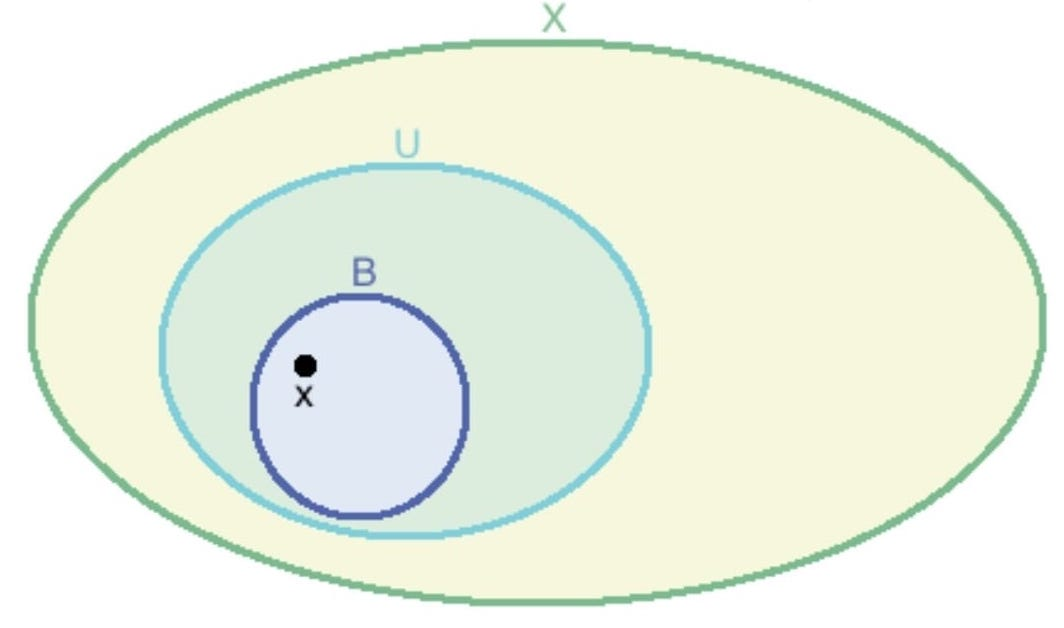
\includegraphics[width=9cm, height=6.5cm]{basis.jpeg}
\end{figure}
    
\end{frame}

\begin{frame}{Quick Recap (contd.)}
    \begin{block}{Closed Set}
    A subset $A$ of a topological space $X$ is said to be closed if $X-A$ is open. 
    \end{block}
    \begin{block}{Product Topology}
    Let $X$ and $Y$ be topological spaces. The product topology on $X \times Y$ is the topology having as basis the collection $\mathscr{B}$ of all sets of the form $U \times V$, where $U$ is an open set of $X$ and $V$ is an open set of $Y$.
    \end{block}
    \begin{block}{Hausdorff Space}
    A topological space $X$ is called a Hausdorff if for each pair of points $x, y \subset X$ such that $x \neq y$, there exist open sets $U$ containing $x$, $V$ containing $y$ such that $U \cap V = \phi$.
    
    \end{block}
\end{frame}

\begin{frame}{Solution to Question 1}
    \begin{block}{Proof}
    For convenience, let us denote $\Delta(X) := \{(x,x) \ | \ x \in X\}$
    
    ($\implies$) We assume that $X$ is a Hausdorff topological space. Showing that $\Delta(X)$ is closed is equivalent to showing that $(X\times X) \setminus \Delta(X)$ is open. 
    
    Let $(x,y) \in (X\times X) \setminus \Delta(X)$. This means that $x \neq y$. Thus, there must exist disjoint open sets $U, V$ of $X$ such that $x \in U, y \in V$. Then, $U \times V$ is an open set in $X \times X$ containing $(x,y)$. To see that $(U \times V) \cap \Delta(X) = \phi$, assume that $(z,z) \subset X\times X$ such that $(z,z) \in (U \times V) \cap \Delta(X)$, which would mean $(z,z) \in U \times V$ which would imply that $U, V$ are not disjoint, a contradiction our assumption.
    \end{block}
    
\end{frame}

\begin{frame}
    \begin{block}{Proof (contd.)}
    ( $\Longleftarrow$ ) Now, we assume that $\Delta(X)$ is closed. 
    
    Let $x \neq y$ be distinct points in X. Then, $(x,y)$ lies in the open set $(X \times X) \setminus \Delta(X)$. We can find an open set $U \times V$ with $(x,y) \in U \times V \subseteq (X\times X) \setminus \Delta(X)$. This implies that $(U \times V) \cap \Delta(X) = \phi$ and thus, $U \cap V = \phi$ proving that X is Hausdorff.  \qedsymbol
    \end{block}
    
\end{frame}

\begin{frame}{Problem 2}
    \begin{block}{Question 11, from Topological Manifolds Section}
     Give an example of an injective smooth map, which is not an immersion.
    \end{block}
   
\end{frame}

\begin{frame}{Quick Recap}
    \begin{block}{Topological Manifold} 
    A topological manifold is a topological space M which is second-countable, locally euclidean and Hausdorff.
    \end{block}
    
    \begin{block}{Chart}
    Let $M$ be a topological $n-$Manifold. A chart on $M$ is a pair $(U,\varphi)$, where $U$ is an open set in $M$ and $\varphi: U \to V$ is a homeomorphism with $V$ being an open set in $\mathbb{R}^n$.
    \end{block}
    
    \begin{block}{Atlas}
    An atlas on $M$ is a collection of charts $\mathscr{A} = \{(U_\alpha,\varphi_{\alpha})\}$ on M such that $\{U_\alpha\}$ cover $M$ and they are mutually compatible: For any pair of indices $\alpha, \beta$, and charts $(U_\alpha,\varphi_{\alpha})$ and $(\ U_{\beta},\varphi_{\beta})$, the map $f_{\beta \alpha} = \varphi_\beta \circ \varphi_\alpha ^{-1}:  \varphi_{\alpha}(U_{\alpha} \cap U_{\beta}) \to \varphi_{\beta}(U_\alpha \cap U_\beta)$ is a homeomorphism. $f_{\beta \alpha}$ is also called a gluing function from chart $i$ to chart $j$. For $M$ to be a smooth manifold, $f_{\beta \alpha}$ is further supposed to be a smooth map.
    \end{block}
    
\end{frame}

\begin{frame}{An Illustration}
\begin{figure}
    \centering
    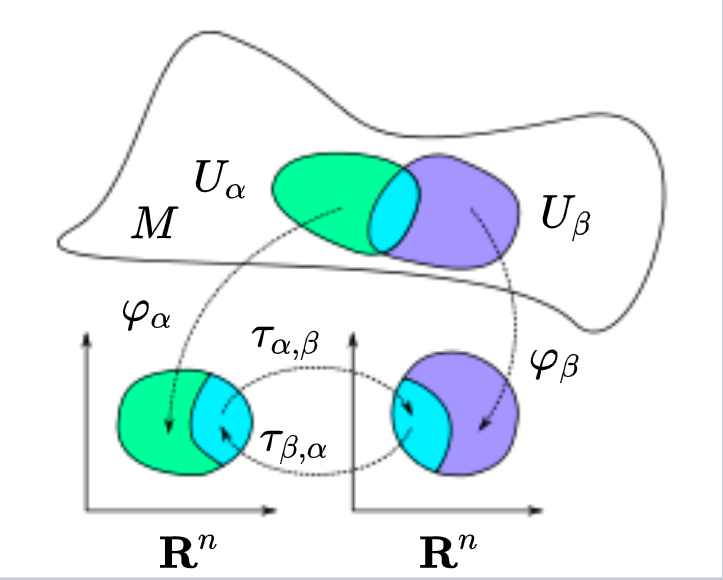
\includegraphics[width=8cm, height=7cm]{gluing_function.png}
\end{figure}
    
\end{frame}

\begin{frame}{Quick Recap (contd.)}
    \begin{block}{Differentiable Manifold}
    For $p \in \mathbb{N} \cup \{\infty\}$, a $p$-fold differentiable manifold is 
    \begin{itemize}
        \item a topological manifold $M$.
        \item an atlas, all whose gluing functions are p times continuously differentiable.
    \end{itemize}
    \end{block}
    
    \begin{block}{Smooth Map}
    A map $f: M \to N$, where $M,N$ are smooth manifolds is called a smooth map if for all pairs of charts $(U,\varphi)$ of $M$ and $(V, \psi)$ of $N$, the map $\varphi^{-1}\circ f \circ \psi: \varphi(U) \to \psi(V)$ is smooth.
    \end{block}
    
    \begin{block}{Immersion Map}
    An immersion is a differentiable function between differentiable manifolds whose derivative is everywhere injective.
    \end{block}
 
\end{frame}

\begin{frame}{Solution to Question 2}
    \begin{block}{Solution/Example}
    Let us consider the set $\mathbb{R}$ with the metric topology. $\mathbb{R}$ is trivially \underline{Hausdorff} and \underline{locally euclidean}. 
    
    The set $\mathscr{C} = \{ (a,b) \subset \mathbb{R} \ | \ a,b \in \mathbb{Q}\}$ is countable and any open set $U$ in $\mathbb{R}$ may be written as a union of a subcollection of $\mathscr{C}$. Thus, $\mathbb{R}$ is \underline{second countable} too. 
    
    This shows that $\mathbb{R}$ is a topological manifold.
    
    We consider the atlas $\mathscr{A} = \{(\mathbb{R}, \varphi_{id})\}$ on $\mathbb{R}$ where $\varphi_{id}: \mathbb{R} \to  \mathbb{R}$ is the identity map. Gluing function for this atlas is trivially the identity map and is thus differentiable. Hence, we can conclude that $\mathbb{R}$ is a differentiable manifold.
    \end{block}
    
\end{frame}

\begin{frame}
    \begin{block}{Solution/Example (contd.)}
    Now, consider the map $f: \mathbb{R} \to \mathbb{R}$ given by $t \to t^3$
    
    $f$ is a smooth map defined between differentiable manifolds, and is an injective function. However, the derivative map is $f': \mathbb{R} \to \mathbb{R}$ given by $t \to 3t^2$ is not injective and thus, $f$ is not an immersion. \qedsymbol
    \end{block}
    
\end{frame}









%---------------------------------------------------------
\section{Atharva Pangarkar, 170110004}
\begin{frame}{Question 1}
\begin{block}{Question 12, from Topological Manifolds Section}
Is the open n-ball diffeomorphic to $\R^n$? 
\end{block}

\end{frame}
\begin{frame}{Prerequisites for Question 1}
\begin{block}{Definition}
Given two smooth manifolds $M \text{ and } N$, $f: M \to N$ is called a diffeomorphism if it is a bijection, it is differentiable and its inverse $f^{-1}:N \to M$ is differentiable as well. If $f$ and $f^{-1}$ are $r$-times continuously differentiable, then $f$ is called a $C^r$ - diffeomorphism. 
\end{block} 
    
\end{frame}
\begin{frame}{Solution to Question 1}
\begin{block}{Solution}
The answer to the question posed is \alert{yes}. We will construct an explicit diffeomorphism from the unit open n-ball denoted as $B^n$ to $\R^n$. This is sufficient because an open n-ball of any radius is diffeomorphic to the unit n-ball due to scaling.

Explicitly, $B^n = \{x \in \R^n: \norm{x} < 1\}$

\textbf{Claim:} The map $\Phi: B^n \to \R^n$ given by \[ x \mapsto \dfrac{x}{\sqrt{1-{\norm{x}}^2}} \] is a diffeomorphism with inverse $\Psi:\R^n \to B^n$ given by \[y \mapsto \dfrac{y}{\sqrt{1+{\norm{y}}^2}} \]. 
\end{block}

\end{frame}

\begin{frame}
\begin{block}{Proof}
The map $\Phi: B^n \to \R^n$ can be written as \[\Phi(x) = \phi(\:\norm{x})\; \dfrac{x}{\norm{x}}\] 
where $\phi:[0,1) \to [0, \infty)$ is given by \[t \mapsto \dfrac{t}{\sqrt{1-t^2}} \]
Put \[ f(x) = \begin{cases}
 \dfrac{\phi(\:\norm{x})}{\norm{x}} & x \neq 0 \\
1 & x = 0 
\end{cases}\] Thus $\Phi(x) = f(x)x$. Note that $f$ is a differentiable function because it is the composition of two differentiable functions as well as the quotient of two differentiable functions. 
\end{block} 
\end{frame}

\begin{frame}
    \begin{block}{Proof (contd.)}
    Now, fixing a standard basis for $\R^n$, we see that $\Phi(x) = (x_1f(x), \ldots, x_nf(x))^T$. Each co-ordinate of $\Phi(x)$ is differentiable, given any $x \in B^n$. Since each coordinate of $\Phi(x)$ is differentiable, the function $\Phi$ is differentiable as well. 
    
    The inverse function of $\Phi$, denoted by $\Psi$ can be written as \[\Psi(y) =\psi(\:\norm{y})\dfrac{y}{\norm{y}} \] where $\psi:[0, \infty) \to [0,1)$ is the inverse function of the scalar valued function $\phi$ and is defined as \[s \mapsto \dfrac{s}{\sqrt{1+s^2}}\]
    
    The relations $\Phi \circ \Psi = \mathrm{ id_{\R^n}}$ and $\Psi \circ \Phi = \mathrm{ id_{B^n}}$ are true. Here $\mathrm{id_A}$ is the identity map on an arbitrary set $A$. This proves that both the functions $\Phi$ and $\Psi$ are bijective. 
    \end{block}
    
\end{frame}
\begin{frame} 
\begin{block}{Proof (contd.)}
The differentiablity of the function $\Psi$ can be proven by the same argument we used to prove the differentiability of $\Phi$. 
    
Finally, we have proven that given the two smooth manifolds $B^n$ and $\R^n$, the function $\Phi: B^n \to \R^n$ is a differentiable map, it is bijective and its inverse is also differentiable. Hence the claim stands proved. \qedsymbol 
\end{block}

\end{frame}

\begin{frame}{Question 2}
\begin{block}{Question 12, from Topology Section}
Suppose $Y$ is an open set in a topological space $X$. Show that: A subset of
$Y$ is open in the subspace topology if and only if it is open in $X$.
\end{block} 
    
\end{frame}

\begin{frame}{Prerequisites for Question 2}
\begin{block}{Definition:}
Given a topological space $(X, \tau)$ and a subset Y of X, the subspace topology on Y is defined as \[\tau_y = \{Y \cap U : U \in \tau \}.\]
That is, a subset of $Y$ is open in the subspace topology of $Y$ if and only if it is the intersection of $Y$ and an open set in $(X, \tau)$. 
\end{block} 
\end{frame}

\begin{frame}{Solution to Question 2}
\begin{block}{Proof}
Let $(X, \tau)$ and $(Y, \tau_y)$ be the spaces given in the question. 

($\Rightarrow$ direction) Let $A$ be a subset open in the subspace topology of $Y$. Then there exists a $U \in \tau$ such that $A = Y \cap U$. It is given to us that $Y$ is open in $X$. Thus $Y \in \tau$ by definition of $\tau$. 
And the intersection of two elements of $\tau$ also lies in $\tau$, again by definition of topology. 
Thus $A = Y \cap U \in \tau$. This implies that $A$ is open in $X$. 

($\Leftarrow$ direction) Suppose $A \subset Y$ is open in X. Thus $A \in \tau$. 

$A = A \cap Y$ since $A \subset Y$. Thus $A \in \tau_y$, by definition of $\tau_y$. Hence $A$ is open in the subspace topology of $Y$. \qedsymbol 

\end{block}
\end{frame}

%---------------------------------------------------------
\section{Nishtha Sinha, 19B090006}

\begin{frame}
\frametitle{Question 1}
\begin{block}{Question}
Show by elementary means that $\mathbb{R}$ and $\mathbb{R}^n$ are not homeomorphic, for $n>1$.
\end{block}
\end{frame}

\begin{frame}{Proof of Question 1}
\begin{block}{Proof}
We proceed via contradiction.\\
Suppose that $\mathbb{R}$ is homeomorphic to $\mathbb{R}^n$. Then by definition, there exists a homeomorphism $f : \mathbb{R} \to \mathbb{R}^n$. \\
Let $A = R \backslash \{0\}$ and observe that 
\begin{align*}
    f|_{A} : R \backslash \{0\} \to \mathbb{R}^n \backslash \{f(0)\}
\end{align*} is also a homeomorphism. In particular, this means that $f_{A}^{-1}$ is continuous. Observe that $f_{A}^{-1} (\mathbb{R}^{n} \backslash \{f(0)\}) = \mathbb{R} \backslash \{0\} $, but $\mathbb{R}^n \backslash \{0\}$ is connected, so $\mathbb{R} \backslash \{0\}$ must be connected since $f_{A}^{-1}$
is continuous by hypothesis. This is a contradiction since $\mathbb{R} \backslash \{0\}$ is not connected ($\mathbb{R} \backslash \{0\} = (-\infty, 0) \cup (0, \infty))$
\end{block}

\end{frame}

\begin{frame}{Question 2}
\begin{block}{Question 14, From Topological Manifolds Section}
Show that $|x|$ is not a sub-manifold of $\R^{2}$
\end{block}
\end{frame}
\begin{frame}{Solution to Question 2}
    \begin{block}{Proof}
    We prove this by contradiction.
    If $(x,|x|)$ were a submanifold of $\mathbb{R}$ x $\mathbb{R}$, there should exist a smooth immersion \(i \) which maps from 
\( ( - \epsilon,  \epsilon) \) to $\mathbb{R}$ x $\mathbb{R}$ with the property that \( i( - \epsilon, \epsilon) = V\). \\
    If so, then \( i(t) = a(t), |a(t|)\) and supposing \( i(0) = (0,0) \), we check the derivative of \(a \) at \( t = 0\). The derivative exists because \( i\) is smooth. \\
    Thus, $\lim_{\delta \to 0} (a( \delta) / \delta) $ becomes \( |a'(0)| \) if \( \delta > 0 \) and  \( -|a'(0)| \) if \( \delta < 0 \). 
	Hence, \( i'(0) = (0,0) \) and therefore, \(i\) can not be an immersion. \qedsymbol
    \end{block}
\end{frame}
%---------------------------------------------------------
\section{Amisha Jangra, 19B090003}
\begin{frame}
\frametitle{Question 1(i)}
\begin{block}{Question 2(i), from Topological Manifolds Section}
Show that: Every subspace of a second countable topological space is second countable. 
\end{block}
\end{frame}


\begin{frame}{Prerequisites for Question 1(i)}
   \begin{block}{Definition} Let $X$ be a topological space. Then, \textit{X} is second countable if it has a countable basis. (That is, \textit{X} has a countable collection of open sets with the property that each open set of \textit{X} is a union of elements in this collection.)
   \end{block}
   \end{frame}
   \begin{frame}
   \frametitle{Solution to Question 1(i)}
   \begin{block}{Solution}
   Let \textit{X} be second countable space, and $A$ be a subspace of $X$. If $\mathscr{B}$ is a countable basis for \textit{X}, then $\{B \cap A | B \in \mathscr{B}\}$ is a countable basis for the subspace \textit{A} of \textit{X}.\\Thus \textit{A} is second countable as well. \qedsymbol
   \end{block}
  
\end{frame}


\begin{frame}
\frametitle{Question 1(ii)}
\begin{block}{Question 2(ii), from Topological Manifolds Section}
Show that : Every subspace of a Hausdorff topological space is Hausdorff.
\end{block}

\end{frame}
\begin{frame}{Prerequisites for Question 1(ii)}
 \begin{block}{Definition}Let \textit{X} be a topological space. Then, \textit{X} is Hausdorff if for any distinct points $x, y \in X$, there exist neighborhoods of \textit{x} and \textit{y} which are disjoint.
 \end{block} 
 \end{frame}
 
 \begin{frame}{Solution}
 \begin{block}{Proof}
 Let $Y$ be a subspace of a Hausdorff space \textit{X}, and let \textit{x} and \textit{y} be two distinct points in the subspace \textit{Y} of \textit{X}. So, we have two disjoint neighborhoods of \textit{x} and \textit{y}, say \textit{U} and \textit{V} respectively. Then, $U \cap Y$ and $V \cap Y$ (both open) are disjoint neighborhoods of \textit{x} and \textit{y} in \textit{Y}. \\
Thus $Y$ is Hausdorff. \qedsymbol
 \end{block}

\end{frame}
\begin{frame}
\frametitle{Question 2}
\begin{block}{Question 5, from Topological Manifolds Section}
The topologist’s sine curve is connected but not path-connected, so it cannot be a topological manifold. Which of the three defining conditions does it violate?
\end{block}
\end{frame}


\begin{frame}{Solution to Question 2}

\begin{block}{Solution}
\begin{align*}
 \Gamma = \{(x, y) : 0 < x \leq 1, y = \sin(1/x)\} \cup \{(0, y) : |y| \leq 1\}
\end{align*}
For $\Gamma$ to be a manifold, it must be Hausdorff, second countable and locally euclidean.\\
\textcolor{blue}{Claim : $\Gamma$ is not locally euclidean.}
\end{block}

\begin{block}{Proof of Claim}
If $\Gamma$ were locally euclidean, then by definition, the point $p=(0,0)$ must have a neighborhood which is homeomorphic to $\mathbb{R}^n$ for some $n \in \mathbb{N}$. And homeomorphism preserves path connectedness, which would imply that $\Gamma$ is path connected, since $\mathbb{R}^n$ is connected, which is a contradiction.
\end{block}
\end{frame}


\begin{frame}{$\Gamma$ is connected}
\begin{block}{Proof (contd.)}
If 
\begin{align*}
S={x \times \sin(1/x) : 0 < x \leq 1}
\end{align*}
then $S$ is the image of the connected set $(0,1]$ under a continuous map, hence $S$ is connected.\\ And the topologist's sine curve is $(0\times [-1,1]) \cup S = \overline{S}$ and since, the closure of a connected set is connected, $\Gamma$ is connected.
\end{block}
\end{frame}



\begin{frame}
\begin{block}{Proof (that $\Gamma$ is not path connected)}
Suppose $f(t) = (a(t), b(t))$ is a continuous curve defined on $[0, 1]$ with $f(t) \in \Gamma$ for all $t > 0$ and $f(0) = (0, 0)$.  \\
\textcolor{blue}{We will try to construct a sequence $\{t_{n}\} \to 0$ such that $b(t_{n}) = (-1)^n$. This will lead to a contradiction, as $f$ is continuous, by assumption}.\\
Take $t_{0} = 1$. \textcolor{green}{So, $f(t_{0}) \in \Gamma$}.
Then by the intermediate value theorem there is a $t_{1}$ such that $0 < t_{1} < 1$ so that $a(t_{1}) = 2/3\pi$. Then there is $0 < t_{2} < t_{1}$ so that $a(t_{2}) = 2/5\pi$. \\ Continuing, we get a decreasing sequence $\{t_{n}\}$ so that $a(t_{n}) = 2/(2n+1)\pi$. It follows that $b(t_{n}) = (-1)^n$.
Now since $\{t_{n}\}$ is a decreasing sequence bounded from below it tends to limit $t_{n} \to 0$. Since $f$ is continuous, $\lim_{n \to \infty} f(t_{n})$ must exist. But $\lim_{n\to \infty} b(t_{n})$ does not exist.\\
\textcolor{green}{We could not get a path connecting $f(t_{0})$ and $f(0)$}.
Therefore $\Gamma$ is not path-connected.
\end{block}
\tiny \textcolor{green}{Green Text - Changes made after presentation}
\end{frame}


%---------------------------------------------------------
\section{Sanjyot Shenoy, 18B030023}


\begin{frame}{Question 1}
\begin{block}{Question 3, from Topological Manifolds Section}
Show that a topological space $\displaystyle X$ is locally $n$-euclidean iff$\displaystyle ( \Leftrightarrow )$ every point $\displaystyle x\in X$ has a neighborhood homeomorphic to an open set of $\displaystyle \mathbb{R}^{n}$.
\end{block}
\end{frame}

\begin{frame}{Prerequisites for Question 1}
Let us recall the concepts required for this question.
\begin{block}{Locally $\displaystyle n$-euclidean}
A topological space $\displaystyle X$ is \alert{locally $n$-euclidean} if every point of $\displaystyle X$ has a neighborhood homeomorphic to $\displaystyle \mathbb{R}^{n}$ for some $\displaystyle n$.
Equivalently $\displaystyle X$ is locally euclidean iff every point of $\displaystyle X$ has a neighborhood homeomorphic to an open $\displaystyle n$-ball for some $\displaystyle n$.
\end{block} 
where open $\displaystyle n$-ball of radius $\displaystyle r$ around $\displaystyle x_{0} \in \mathbb{R}^{n}$ is $\displaystyle B^{n}( x_{0} ,r) =\left\{x\in \mathbb{R}^{n} \ |\ ||x_{0} -x||< r\right\}$ 
\begin{block}{Homeomorphism}
Let $\displaystyle X,Y$ be two topological spaces. A bijective map $\displaystyle f:X\rightarrow Y$ is said to be a \alert{homeomorphism} if $\displaystyle f$ and $\displaystyle f^{-1}$ are continuous. 
\end{block}
\end{frame}
\begin{frame}{Prerequisites for Question 1 (contd.)}
\begin{block}{Open Set in Metric Topology}
A subset $\displaystyle U$ of a metric space $\displaystyle X$ is open (in the metric topology) if $\displaystyle \forall x\in U$, there exists a $\displaystyle r >0$ such that $\displaystyle B( x,r) \subseteq U$.
\end{block}
\end{frame}
\begin{frame}{Sketch of Proof}
We have a two-way traffic ($\displaystyle \Leftrightarrow $) here. 

First we note that, the $\displaystyle \Rightarrow $ direction follows from definition of locally $\displaystyle n$-euclidean spaces. 

\alert{The trouble lies in proving the converse!}
\end{frame}
\begin{frame}{Sketch of Proof (contd.)}
Now, for the converse ($\displaystyle \Leftarrow $) part,

For each point \ $\displaystyle x\in X$ \ we have a neighborhood, $\displaystyle V_{x}$ say, homeomorphic to an open set, let's say $\displaystyle U_{x}$ of $\displaystyle \mathbb{R}^{n}$. 

From this information, we need to construct a homeomorphism from an open neigbourhood of $\displaystyle x$ to either $\displaystyle \mathbb{R}^{n}$ or an open $\displaystyle n$-ball 

How to go about this? 

We will use two facts 
\begin{enumerate}
\item open $\displaystyle n$-balls form a basis for topology on $\displaystyle \mathbb{R}^{n}$, and hence are open, 
\item definition of an open set in a metric space 
\end{enumerate}

Then restrict ourselves to an open $\displaystyle n$-ball inside the open set, then trace it back to its domain in $\displaystyle X$ 
\end{frame}
\begin{frame}{Diagram}
\begin{figure}
    \centering
    \centering
    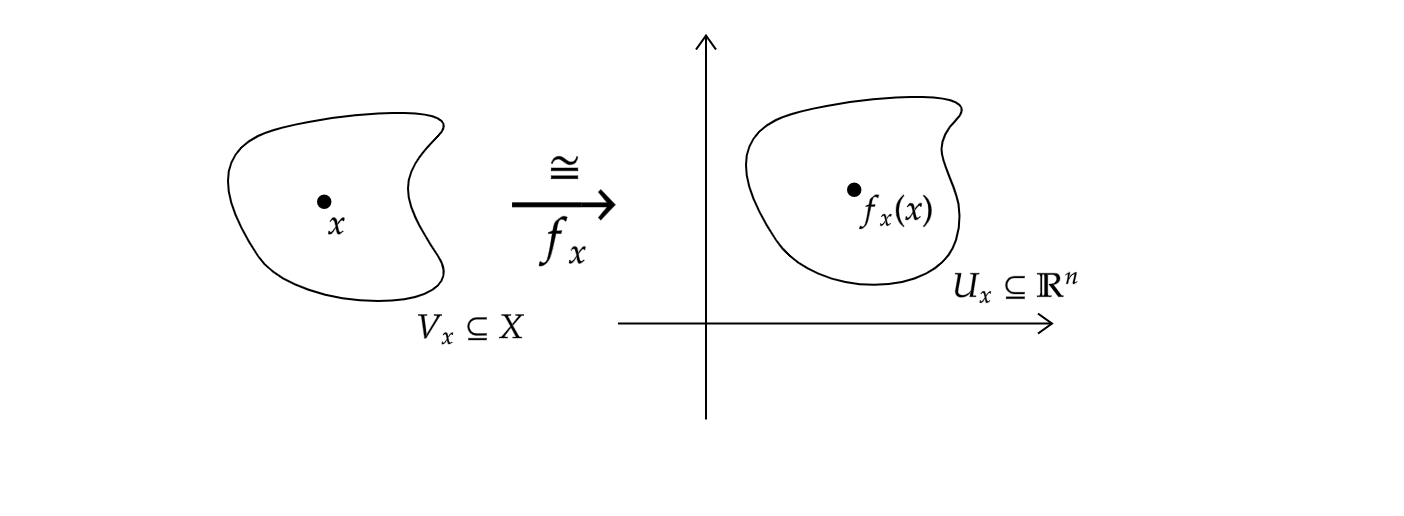
\includegraphics[width = 1.1\textwidth]{diag-1.png}

    %\includegraphics{}
    %\label{fig:my_label}
\end{figure}
Note here the subscripts represent that the functions and the sets \alert{depend} on $x$.
\end{frame}
\begin{frame}{Proof of Question 1}
Now we get to the explicit details. 
\begin{block}{Proof}
($\displaystyle \Rightarrow $): Here $\displaystyle X$ is locally $\displaystyle n$-euclidean, hence, by our criterion, for each $\displaystyle x\in X$, we have a neighbourhood homeomorphic to $\displaystyle \mathbb{R}^{n}$. Since $\displaystyle \mathbb{R}^{n}$ is an open set in $\displaystyle \mathbb{R}^{n}$, we are done. 

Equivalently, $\displaystyle X$ is locally $\displaystyle n$-euclidean, hence, for each $\displaystyle x\in X$, we have a neighbourhood homeomorphic to an open $\displaystyle n$-ball, and since open $\displaystyle n$-balls are open sets in \ $\displaystyle \mathbb{R}^{n}$, we are done. 
\end{block}
\end{frame}
\begin{frame}
\begin{block}{Proof(contd.)}
($\displaystyle \Leftarrow $): Let us suppose that for each $\displaystyle x\in X$, we have a neighborhood $\displaystyle V_{x}$ \ homeomorphic to an open set $\displaystyle U_{x} \subseteq \mathbb{R}^{n}$, via the homeomorphism $\displaystyle f_{x}$.  

Since $\displaystyle U_{x}$ is an open set in $\displaystyle \mathbb{R}^{n}$, which is a metric space, and we have $\displaystyle f_{x}( x) \in U_{x}$, then, there exists an open $\displaystyle n$-ball $\displaystyle B( f_{x}( x) ,r)$ such that $\displaystyle B( f_{x}( x) ,r) \subseteq U_{x}$. 


Since $\displaystyle f_{x}$ is a homeomorphism $\displaystyle \Rightarrow $ $\displaystyle f_{x}^{-1}( B( f_{x}( x) ,r))$ is an open set in $\displaystyle X$. Let $\displaystyle V'_{x} =f_{x}^{-1}( B( f_{x}(x),r))$. Clearly, $\displaystyle x\in V'_{x}$, since $\displaystyle f_{x}( x) \in B( f_{x}(x),r)$. Thus $\displaystyle V'_{x}$ is a neighbourhood of $\displaystyle x$. 

Consider the restriction, $\displaystyle h_{x}$ of $\displaystyle f_{x}$ to $\displaystyle V'_{x}$, that is $\displaystyle h_{x} =f_{x} |_{V'_{x}} :\ V'_{x}\rightarrow B( f_{x}( x) ,r)$, then

\textbf{Claim}: $\displaystyle h_{x}$ is a homeomorphism. 

\textbf{Proof of Claim}: Since $\displaystyle f_{x}$ is bijective on $\displaystyle V_{x}$, it in injective on $\displaystyle V'_{x}$, surjectivity follows since$\displaystyle V'_{x} =f_{x}^{-1}( B( x,r))$. Continuity of $\displaystyle h_{x}$ follows from continuity of $\displaystyle f_{x}$ and similarly for $\displaystyle h_{x}^{-1}$. 

Hence for each $\displaystyle x\in X$, we have a neigbourhood which is homeomorphic to an open $\displaystyle n$-ball, hence, $\displaystyle X$ is locally $\displaystyle n$-euclidean. $\displaystyle \qed $ 
\end{block}
\end{frame}
\begin{frame}{Diagram}
\begin{figure}
    \centering
    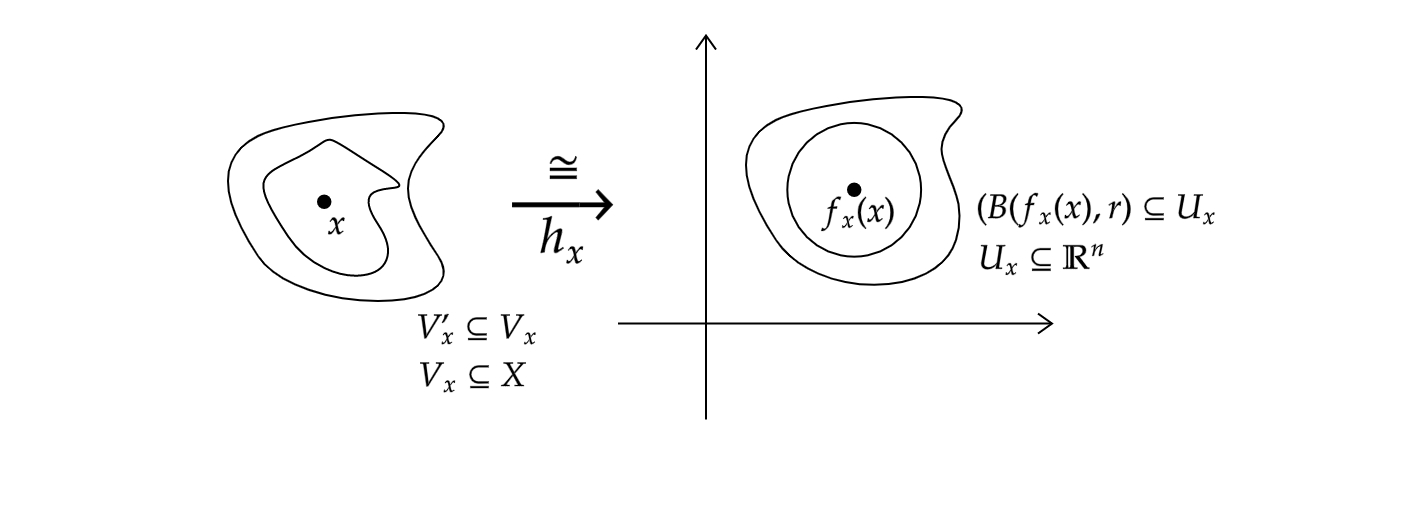
\includegraphics[width = 1.1\textwidth]{diag-2.png}
    \caption{A pictorial view of the construction}
\end{figure}
\end{frame}


\begin{frame}{Question 2}
\begin{block}{Question 4, from Topological Manifolds Section}
Consider the three conditions on a topological space in the definition of a topological manifold. Think of examples which satisfy two of those conditions
but not the third.
\end{block}
\end{frame}

\begin{frame}{Prerequisites for Question 2}
Let $X$ be a topological space.
\begin{block}{Second Countable}
$\displaystyle X$ is \alert{second countable} if it has a countable basis. 
\end{block}
\begin{block}{Locally $n$-euclidean}
A topological space $\displaystyle X$ is \alert{locally $n$-euclidean} if every point of $\displaystyle X$ has a neighborhood homeomorphic to $\displaystyle \mathbb{R}^{n}$ for some $\displaystyle n$.


Equivalently $\displaystyle X$ is locally
euclidean iff every point of $\displaystyle X$ has a neighborhood homeomorphic to an open $\displaystyle n$-ball for some $\displaystyle n$.


\end{block}
\begin{block}{Hausdorff Space}
$\displaystyle X$ is \alert{Hausdorff} if for any distinct points $\displaystyle x,y\in X$, there exist neighborhoods of $\displaystyle x$ and $\displaystyle y$ which are disjoint.
\end{block}
\end{frame}
\begin{frame}{Prerequisites for Question 2 (contd.)}
\begin{block}{Topological Manifold}
$\displaystyle X$ is a topological manifold if it is Hausdorff, second countable, and locally $\displaystyle n$-euclidean for some $\displaystyle n$.
\end{block}
\end{frame}
\begin{frame}{Solution to Question 2}
\begin{exampleblock}{Example 1: Hausdorff and Second Countable but not locally euclidean}
$\displaystyle X=[ 0,1] \subseteq \mathbb{R}$, with the subspace topology. Then, $\displaystyle X$ is Hausdorff, since $\displaystyle \mathbb{R}$ is Hausdorff. It is also second coutable since $\displaystyle \mathbb{R}$ is. 

However it is not locally euclidean! 

To see this, note that, $\displaystyle ( 0,1) \subseteq \mathbb{R}$ under subspace topology is locally $\displaystyle 1$-euclidean, hence we will try to see if $\displaystyle X$ is locally $\displaystyle n$-euclidean, for $\displaystyle n=1$, $\displaystyle n >1$ is not possible, since if it is, then $\displaystyle ( 0,1)$ will also be $\displaystyle n$-euclidean for this $\displaystyle n$, which is not possible, as $\displaystyle ( 0,1) =B\left(\frac{1}{2} ,\frac{1}{2}\right)$, which cannot be homeomorphic to any open set in $\displaystyle \mathbb{R}^{n}$ as a consequence of invariance of domain theorem of Brouwer.

\end{exampleblock}
\end{frame}
\begin{frame}{Solution to Question 2 (contd.)}
\begin{exampleblock}{Example 1(contd.)}
Suppose, $\displaystyle X$ is locally $\displaystyle 1$-euclidean, then every for every point in $\displaystyle X$, it has a neighbourhood which is homeomorphic to a $\displaystyle 1$-ball, which is a an interval in $\displaystyle \mathbb{R}$. 

Then, this should hold for $\displaystyle 0$ and $\displaystyle 1$ as well. Note that open neigbourhoods of $\displaystyle 0$ and $\displaystyle 1$ in $\displaystyle X$ look like $\displaystyle [ 0,a)$ and $\displaystyle ( b,1]$, where $\displaystyle a,b\in ( 0,1)$, respectively, which are half intervals. Half intervals are not homeomorphic to open intervals, and thus $\displaystyle X$ is not locally $\displaystyle 1$-euclidean, and not thus not locally euclidean. 
\end{exampleblock}  
\end{frame}
\begin{frame}{Solution to Question 2 (contd.)}
\begin{alertblock}{Example 2: Locally Euclidean and Second Countable but not Hausdorff}
One of such examples is the real line with two origins. 

Explicitly,

It is the quotient space of two copies of real line, obtained by identifying any two points with same $\displaystyle x$-coordinate, that is 
\begin{equation*}
\mathbb{R} \times \{a\}\text{ and }\mathbb{R} \times \{b\}
\end{equation*}
with equivalence relation defined by 
\begin{equation*}
( x,a) \sim ( x,b) ,\ \text{if} \ x\neq 0
\end{equation*}
Pictorially this looks like:
\end{alertblock}  
\end{frame}


\begin{frame}{Solution to Question 2 (contd.)}
\begin{alertblock}{Example 2(contd.)}
\begin{figure}
    \centering
    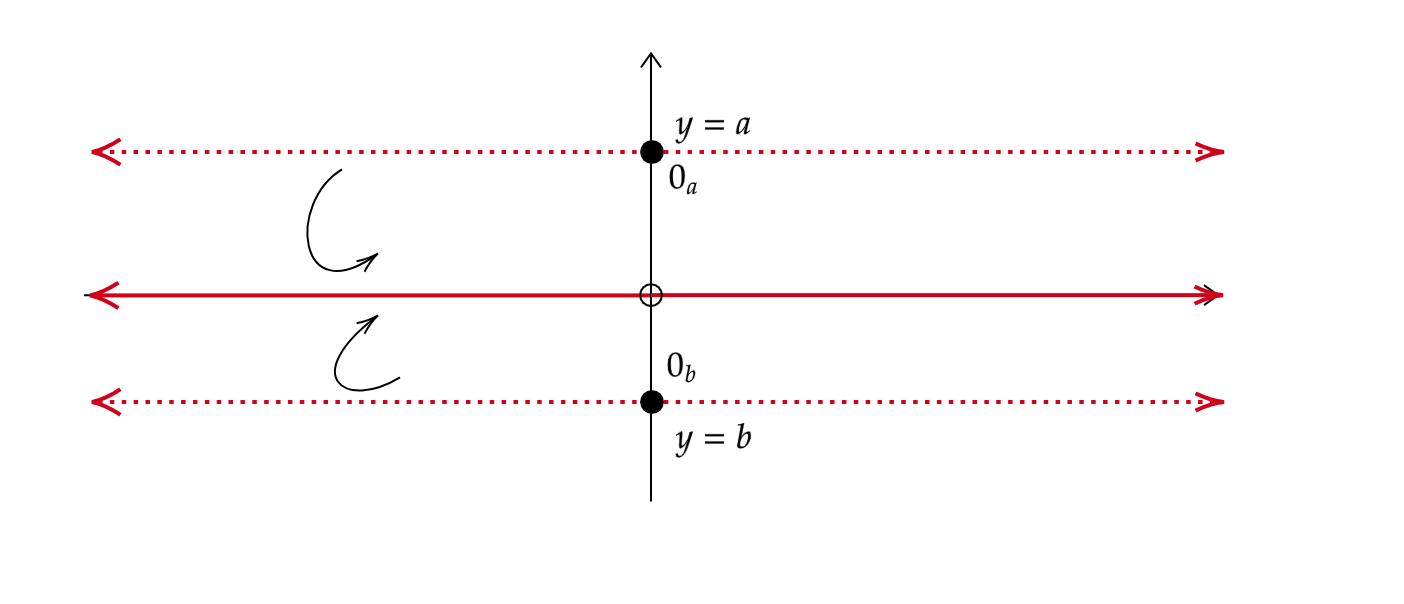
\includegraphics[width = 1.1\textwidth]{diag-3.png}
    \caption{A pictorial view of the construction}
\end{figure}

\end{alertblock}  
\end{frame}

\begin{frame}{Solution to Question 2 (contd.)}
\begin{alertblock}{Example 2(contd.)}
Thus, we have that, for $\displaystyle x=0$, two points, denoted by $\displaystyle 0_{a}$ and $\displaystyle 0_{b}$. Any neigbourhood of $\displaystyle 0_{a}$ looks like  

$\displaystyle B( 0_{a} ,\epsilon ) =\{r\in \mathbb{R} \backslash \{0\} |-\epsilon < r< \epsilon \} \ $and similarly for $\displaystyle 0_{b}$. Thus, all neighbourhoods intersect, and thus these points cannot be separated, and hence this space is not Hausdorff. 

Second countability and locally $\displaystyle 1$-euclidean property follows from respective properties of $\displaystyle \mathbb{R}$ 
\end{alertblock}  
\end{frame}


\begin{frame}{Solution to Question 2 (contd.)}
\begin{block}{Example 3: Hausdorff and Locally Euclidean, but not second countable.}
Form $\displaystyle X=\mathbb{R} \times \mathbb{R}_{d}$, that is product topology of $\displaystyle \mathbb{R}$ with it's standard topology and $\displaystyle \mathbb{R}$ with it's discrete topology.

It is a topological space under the product topology, it is Hausdorff since both $\displaystyle \mathbb{R}$ and $\displaystyle \mathbb{R}_{d}$ are Hausdorff Spaces.

The discrete topology on $\displaystyle \mathbb{R}$ can be given by the following metric: 
\begin{gather*}
d( x,y) =1,\ x\neq y\\
d( x,y) =0,\ x=y
\end{gather*} 
Thus the only possible balls around a point $\displaystyle x\in \mathbb{R}$ are $\displaystyle \mathbb{R}$ or $\displaystyle \{x\}$, which implies that, $\displaystyle \mathbb{R}_{d}$ is $\displaystyle 0$-euclidean.

It is locally euclidean, since $\displaystyle \mathbb{R}$ is locally euclidean, and so is $\displaystyle \mathbb{R}_{d}$ is locally euclidean. 

However it is not second-countable since $\displaystyle \mathbb{R}_{d}$ is not second countable. 
Pictorially, this looks like:
\end{block}  
\end{frame}

\begin{frame}{Diagram for Example 3}
\begin{block}{Example 3(contd.)}
\begin{figure}
    \centering
    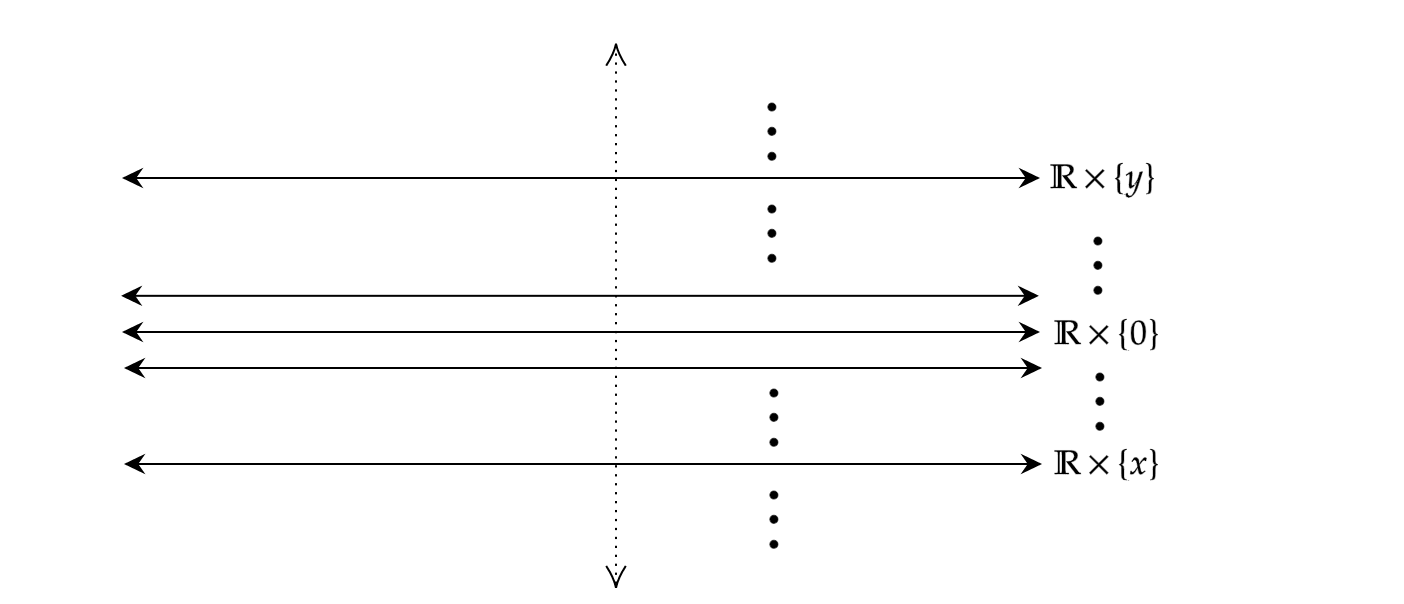
\includegraphics[width = 1.1\textwidth]{diag-4.png}
    \caption{A pictorial view of the space}
\end{figure}
\end{block}
\end{frame}
\begin{frame}{Thank you!}
    Any questions or suggestions?
    
    \alert{Post Presentation Remarks:} \\
    \begin{enumerate}
        \item In Example 3 above, just $\R_{d}$ suffices.
        \item In Example 3 above, I had chosen an example where the space is totally disconnected, so are there spaces with same property but connected? 
    \end{enumerate}
\end{frame}


%---------------------------------------------------------
\begin{frame}{End of Presentation}
        For any corrections/typos, please contact us!\\
        A \alert{big thank you} to \textbf{Prof. Swapneel Mahajan} for this opportunity!
        
    \end{frame}
%---------------------------------------------------------

\end{document}